\documentclass[a4paper,12pt]{article} 
\makeatletter\if@twocolumn\PassOptionsToPackage{switch}{lineno}\else\fi\makeatother

\usepackage{amsfonts,amssymb,amsbsy,latexsym,amsmath,tabulary,graphicx,times,xcolor}
\usepackage[T1]{fontenc}
\usepackage{url,multirow,morefloats,floatflt,cancel,tfrupee,multicol}
\makeatletter

\AtBeginDocument{\@ifpackageloaded{textcomp}{}{\usepackage{textcomp}}}
\makeatother
\usepackage{colortbl}
\usepackage{xcolor}
\usepackage{pifont}
\usepackage{placeins}
\usepackage[nointegrals]{wasysym}
\usepackage[superscript,biblabel]{cite}
\urlstyle{rm}
\makeatletter

%Etal definition in references
\@ifundefined{etal}{\def\etal{\textit{et~al}}}{}

\AtBeginDocument{
\expandafter\ifx\csname eqalign\endcsname\relax
\def\eqalign#1{\null\vcenter{\def\\{\cr}\openup\jot\m@th
  \ialign{\strut$\displaystyle{##}$\hfil&$\displaystyle{{}##}$\hfil
      \crcr#1\crcr}}\,}
\fi
}

\@ifundefined{tsGraphicsScaleX}{\gdef\tsGraphicsScaleX{1}}{}
\@ifundefined{tsGraphicsScaleY}{\gdef\tsGraphicsScaleY{.9}}{}
% To automatically resize figures to fit inside the text area
\def\checkGraphicsWidth{\ifdim\Gin@nat@width>\linewidth
	\tsGraphicsScaleX\linewidth\else\Gin@nat@width\fi}

\def\checkGraphicsHeight{\ifdim\Gin@nat@height>.9\textheight
	\tsGraphicsScaleY\textheight\else\Gin@nat@height\fi}

\def\fixFloatSize#1{}

\let\ts@includegraphics\includegraphics

\def\inlinegraphic[#1]#2{{\edef\@tempa{#1}\edef\baseline@shift{\ifx\@tempa\@empty0\else#1\fi}\edef\tempZ{\the\numexpr(\numexpr(\baseline@shift*\f@size/100))}\protect\raisebox{\tempZ pt}{\ts@includegraphics{#2}}}}


\AtBeginDocument{\def\includegraphics{\@ifnextchar[{\ts@includegraphics}{\ts@includegraphics[width=\checkGraphicsWidth,height=\checkGraphicsHeight,keepaspectratio]}}}

\DeclareMathAlphabet{\mathpzc}{OT1}{pzc}{m}{it}

\def\URL#1#2{\@ifundefined{href}{#2}{\href{#1}{#2}}}

\edef\fntEncoding{\f@encoding}
\def\EUoneEnc{EU1}
\makeatother
\def\floatpagefraction{0.8} 
\def\dblfloatpagefraction{0.8}
\def\style#1#2{#2}
\def\xxxguillemotleft{\fontencoding{T1}\selectfont\guillemotleft}
\def\xxxguillemotright{\fontencoding{T1}\selectfont\guillemotright}

\newif\ifmultipleabstract\multipleabstractfalse%
\newenvironment{typesetAbstractGroup}{}{}%

%%%%%%%%%%%%%%%%%%%%%%%%%%%%%%%%%%%%%%%%%%%%%%%%%%%%%%%%%%%%%%%%%%%%%%%%%%

\usepackage[hmargin=1.8cm,vmargin=2.2cm]{geometry}%,headsep=0.3in,footskip=0.49in
\setlength{\columnsep}{0.25in}
\setlength\headheight{19.5pt}

\makeatletter
\def\author#1{\gdef\@author{\hskip-\dimexpr(\tabcolsep)\hskip1pt\parbox{\dimexpr\textwidth-1pt}{\centering #1}}}

\let\@articletype\@empty \def\articletype#1{\gdef\@articletype{{\fontsize{14}{16}\selectfont #1}}}

\usepackage{fancyhdr}
\renewcommand{\headrulewidth}{0pt}
\renewcommand{\footrulewidth}{0pt}
\fancypagestyle{headings}{\fancyhf{}\fancyhead[RE]{\MakeTextUppercase{\textbf{\RunningAuthor}}}\fancyhead[LE]{\textbf{\thepage}}\fancyhead[LO]{\MakeTextUppercase{\textbf{\RunningHead}}}\fancyhead[RO]{\textbf{\thepage}}}\pagestyle{headings}
\fancypagestyle{plain}{\fancyhf{}\fancyfoot[C]{\textbf{\thepage}}}

\AtBeginDocument{\usepackage{lastpage}}
\def\title#1{
  \gdef\@title{
    \ifx\@articletype\@empty\else\@articletype~\\\fi%
     #1}
}


\usepackage{abstract}
\def\abstractname{\textbf{Abstract}}
\renewenvironment{onecolabstract}
{\vspace*{-.4pc}\trivlist\item[]\leftskip1pt\noindent\selectfont\hfill\abstractname\hfill\mbox{\null}\par\ignorespaces}{\endtrivlist}

\def\NormalBaseline{\def\baselinestretch{1.1}}

\usepackage{textcase}
\usepackage[explicit]{titlesec}
\setcounter{secnumdepth}{5}

\titleformat{\section}[block]{\NormalBaseline\boldmath\bfseries}
{\thesection.}
{6pt}
{#1}
[]
\titleformat{\subsection}[hang]{\NormalBaseline\filright\itshape}
{\thesubsection.}
{6pt}
{#1}
[]
\titleformat{\subsubsection}[runin]{\NormalBaseline\filright\itshape}
{\hspace{16pt}\thesubsubsection}
{6pt}
{#1}
[]
\titleformat{\paragraph}[runin]{\NormalBaseline}
{\theparagraph}
{6pt}
{#1}
[]
\titleformat{\subparagraph}[runin]{\NormalBaseline}
{\thesubparagraph}
{6pt}
{#1}
[]

\titlespacing{\section}{0pt}{1.5\baselineskip}{.2\baselineskip}  
\titlespacing{\subsection}{0pt}{1.5\baselineskip}{.2\baselineskip}  
\titlespacing{\subsubsection}{0pt}{1.5\baselineskip}{.2\baselineskip}  
\titlespacing{\paragraph}{0pt}{.5\baselineskip}{10pt}  
\titlespacing{\subparagraph}{0pt}{.5\baselineskip}{10pt}


\usepackage{caption}
\DeclareCaptionLabelFormat{figlabel}{Figure #2}
\captionsetup[figure]{font={footnotesize},labelfont={bf},labelformat=figlabel,skip=1.4pt,aboveskip=1pc,labelsep=period,justification=centering}
\captionsetup[table]{font={footnotesize},skip=1.4pt,labelsep=period,justification=centering}

\date{}
\makeatother



\usepackage{float}
\usepackage{hyperref}


\setcounter{topnumber}{1}
\setcounter{bottomnumber}{1}
\renewcommand{\topfraction}{0.85}
\renewcommand{\textfraction}{0.1}
\renewcommand{\floatpagefraction}{0.85}
\renewcommand{\topfraction}{0.9}

%%%%%%%%%%%%%%%%%%%%%%%%%%%%%%%%%%%%%%%%%%%%%%%%%%%%%%%%%%%%%%%%%%%%%%%%%%
%% Document content 
%%%%%%%%%%%%%%%%%%%%%%%%%%%%%%%%%%%%%%%%%%%%%%%%%%%%%%%%%%%%%%%%%%%%%%%%%%


\begin{document}

\title{Assignment 01: Basic Image Processing}

\def\RunningHead{
Basic Image Processing
}
\def\RunningAuthor{Basic Image Processing}
\date{Submitted on: December 3, 2024} 

\maketitle

\vspace{-2em} 

\begin{center}
    \textbf{Faculty Name:} Faculty Of Sciences Rabat\\
    \textbf{Master Program:} Intelligent Processing Systems\\
    \textbf{Course Name:} Computer Vision\\
    \textbf{Student Name:} El Mahraoui Amal \\
    \textbf{Lecturer:} El Hajoui Souhaila \\
\end{center}



%%%%%%%%%%%%%%%%%%%%%%%%%%%%%%%%%%%%%%%%%%%%%%%%%%%%%%%%%%%%%%%%%%%%%%%%%%

{\begin{onecolabstract}
This report focuses on applying image processing techniques using MATLAB to enhance image quality and extract meaningful information. Key methods such as dynamic range expansion, histogram equalization, and adaptive histogram equalization were implemented on grayscale images to improve contrast and visibility. By utilizing MATLAB's built-in image processing tools, this study highlights the effectiveness of these techniques in improving image clarity, adjusting contrast, and achieving precise object segmentation, demonstrating their practical value in computer vision and related applications.

\def\keywordstitle{Keywords}
\smallskip\noindent\textbf{Keywords: }{\normalfont
\textit{dynamic range expansion}, \textit{histogram equalization}, \textit{adaptive histogram equalization}.
}
\end{onecolabstract}}
 
%%%%%%%%%%%%%%%%%%%%%%%%%%%%%%%%%%%%%%%%%%%%%%%%%%%%%%%%%%%%%%%%%%%%%%%%%%
\begin{multicols}{2}

\section{Introduction}
Image enhancement plays a key role in improving image quality, especially when captured under challenging conditions such as poor lighting. In computer vision, enhancing images helps with better feature recognition, making it easier to identify and analyze details. This report focuses on three common image enhancement methods: dynamic range expansion, histogram equalization, and adaptive histogram equalization. These techniques are tested on both grayscale and color images to improve contrast and clarity. Additionally, segmentation is explored by isolating objects from their backgrounds, using thresholding methods applied to both enhanced grayscale and color images. 



\section{Methodology}
\subsection{Grayscale Image Processing}
\textbf{Task 1:} Dynamic Range Expansion \\
The images sosie.png and scene.png were processed using MATLAB’s rescale and imadjust functions to expand the pixel intensity range. Histograms were generated before and after processing to assess the effect of dynamic range expansion.

\textbf{Task 2:} Histogram Equalization\\
The histeq function was used on the same images to perform histogram equalization, aiming to redistribute pixel intensities for more uniform contrast. The histograms were compared before and after applying the method to evaluate its effectiveness.

\textbf{Task 3:} Adaptive Histogram Equalization\\
The adapthisteq function was applied to book.png to enhance local contrast in areas with uneven lighting. The results were compared with the binarization technique applied to the original and enhanced images.

\subsection{Color Image Processing}
\textbf{Task 1: } Channel Extraction\\
The image carottes.png was processed to extract the red, green, and blue color channels. These channels were separated using MATLAB’s imsplit function, and histograms were displayed for each extracted channel.

\textbf{Task 2: } Segmentation\\
The imbinarize function was used on the extracted channels with automatic thresholding (graythresh) to isolate the carrots in the image. Manual thresholding was also performed based on histogram analysis to refine the segmentation process.



\section{Results}
\subsection{Grayscale Image Processing}
\textbf{Task 1:} Dynamic Range Expansion\\

%%%%%%%%%%

%%%%%%%%%%%%%%
The dynamic range expansion improved the contrast of both sosie.png and scene.png, stretching the intensity range and making the images appear clearer. However, this method did not enhance details in shadowed areas as effectively as histogram equalization. 
\begin{figure}[H]
    \centering
    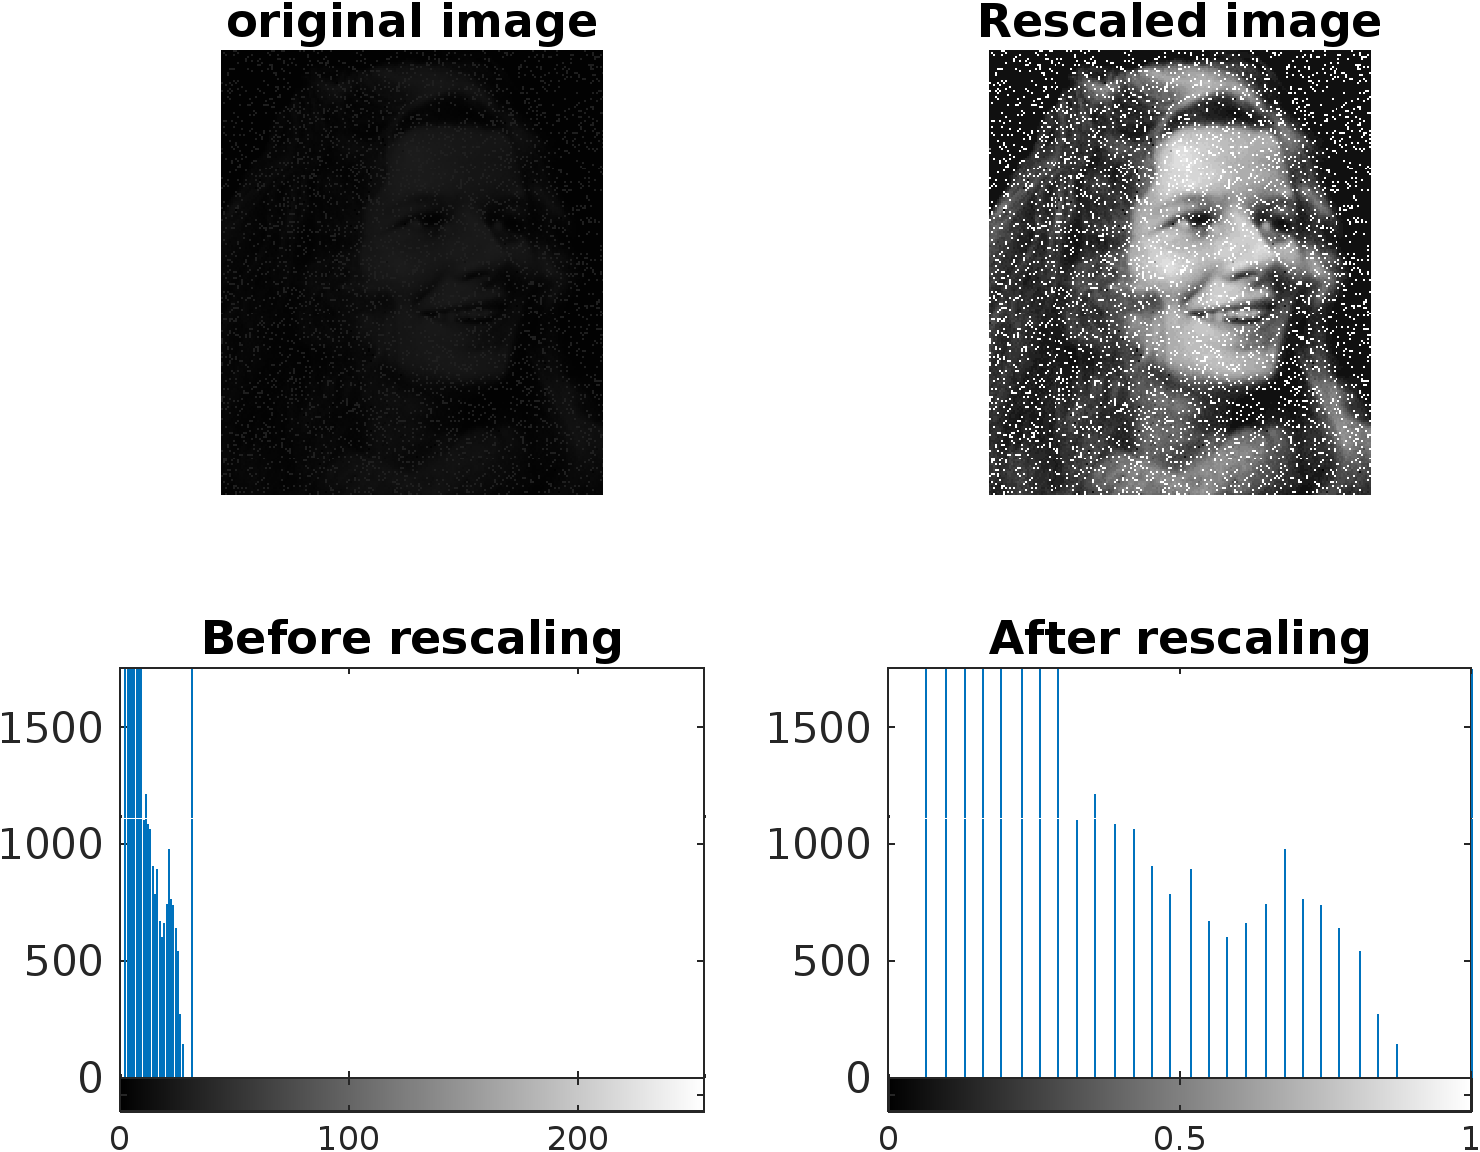
\includegraphics[width=0.50\linewidth]{Images/Figure 1.png} % Replace with your image path
    \caption{Dynamic Range Expansion results on grayscale images(Rescaling).}
    \label{fig:dynamic_range_expansion}
\end{figure}
\begin{figure}[H]
    \centering
    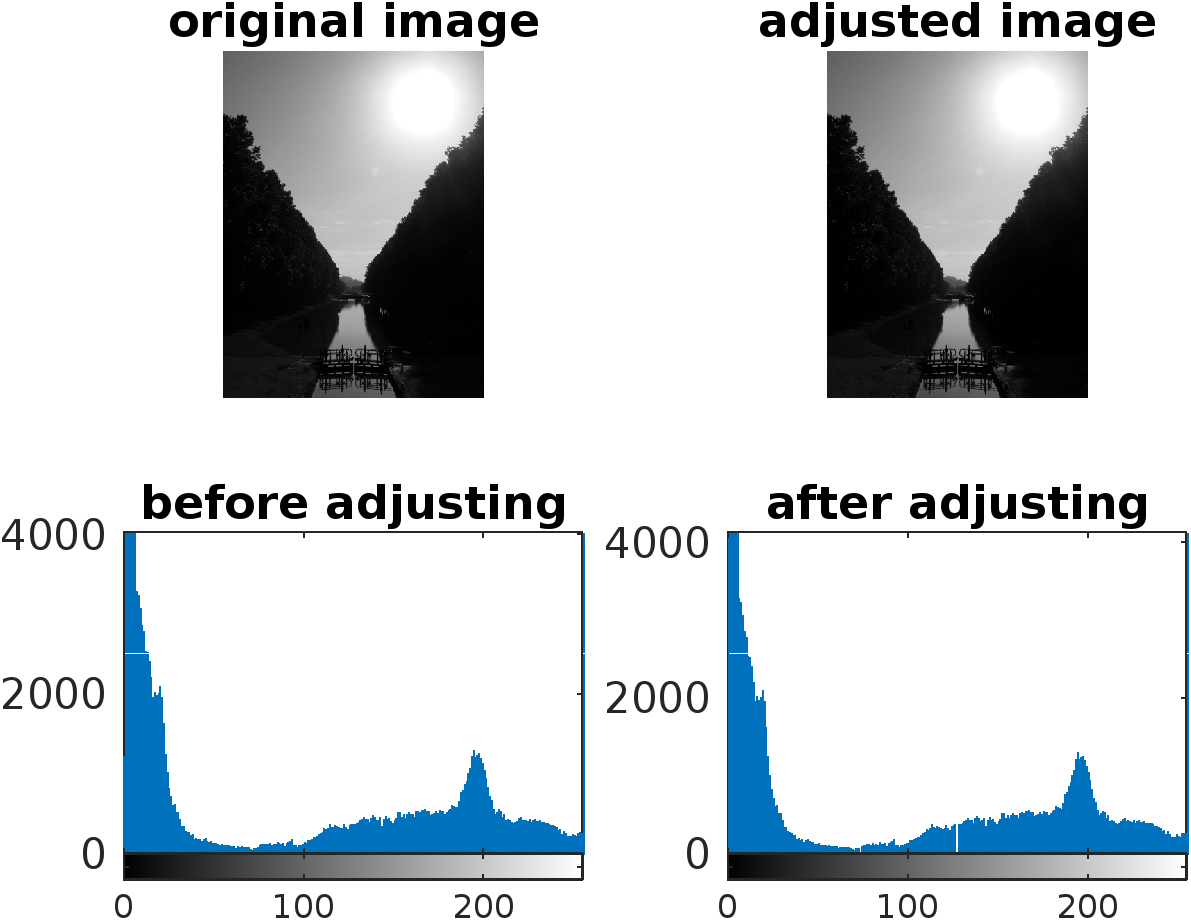
\includegraphics[width=0.50\linewidth]{Images/Figure 4.png} % Replace with your image path
    \caption{Dynamic Range Expansion results on grayscale images (Adjusting).}
    \label{fig:dynamic_range_expansion}
\end{figure}



\textbf{Task 2:} Histogram Equalization\\
Histogram equalization produced more uniform contrast in both images, highlighting details in darker regions that were less visible in the original images. This method improved overall visual quality.
\begin{figure}[H]
    \centering
    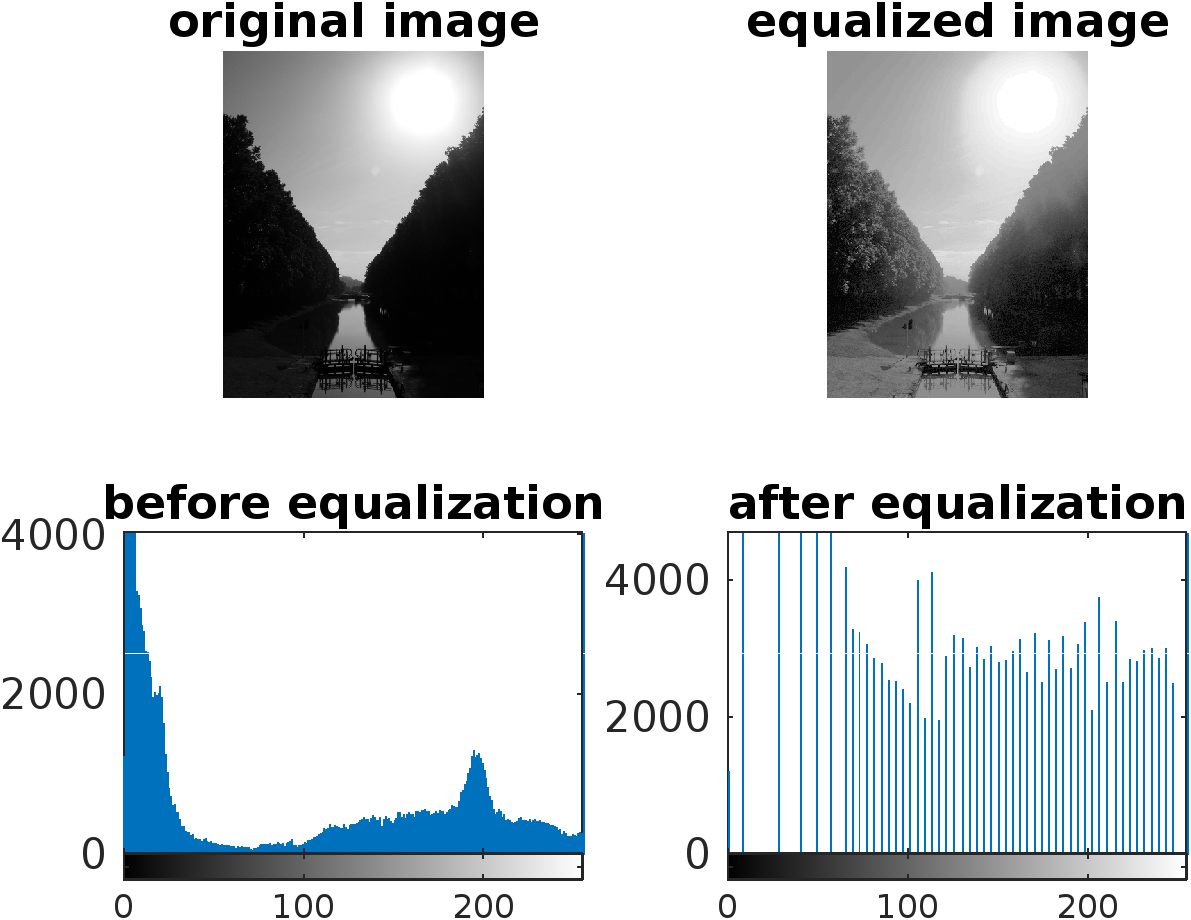
\includegraphics[width=0.50\linewidth]{Images/Figure 6.png} 
    \caption{Histogram Equalization results on grayscale images.}
    \label{fig:dynamic_range_expansion}
\end{figure}

\textbf{Task 3:} Adaptive Histogram Equalization\\
Adaptive histogram equalization significantly enhanced the visibility of text and details in shadowed regions of book.png. The binarization of the original image and enhanced images showed improved segmentation in comparison to the other methods.
\begin{figure}[H]
    \centering
    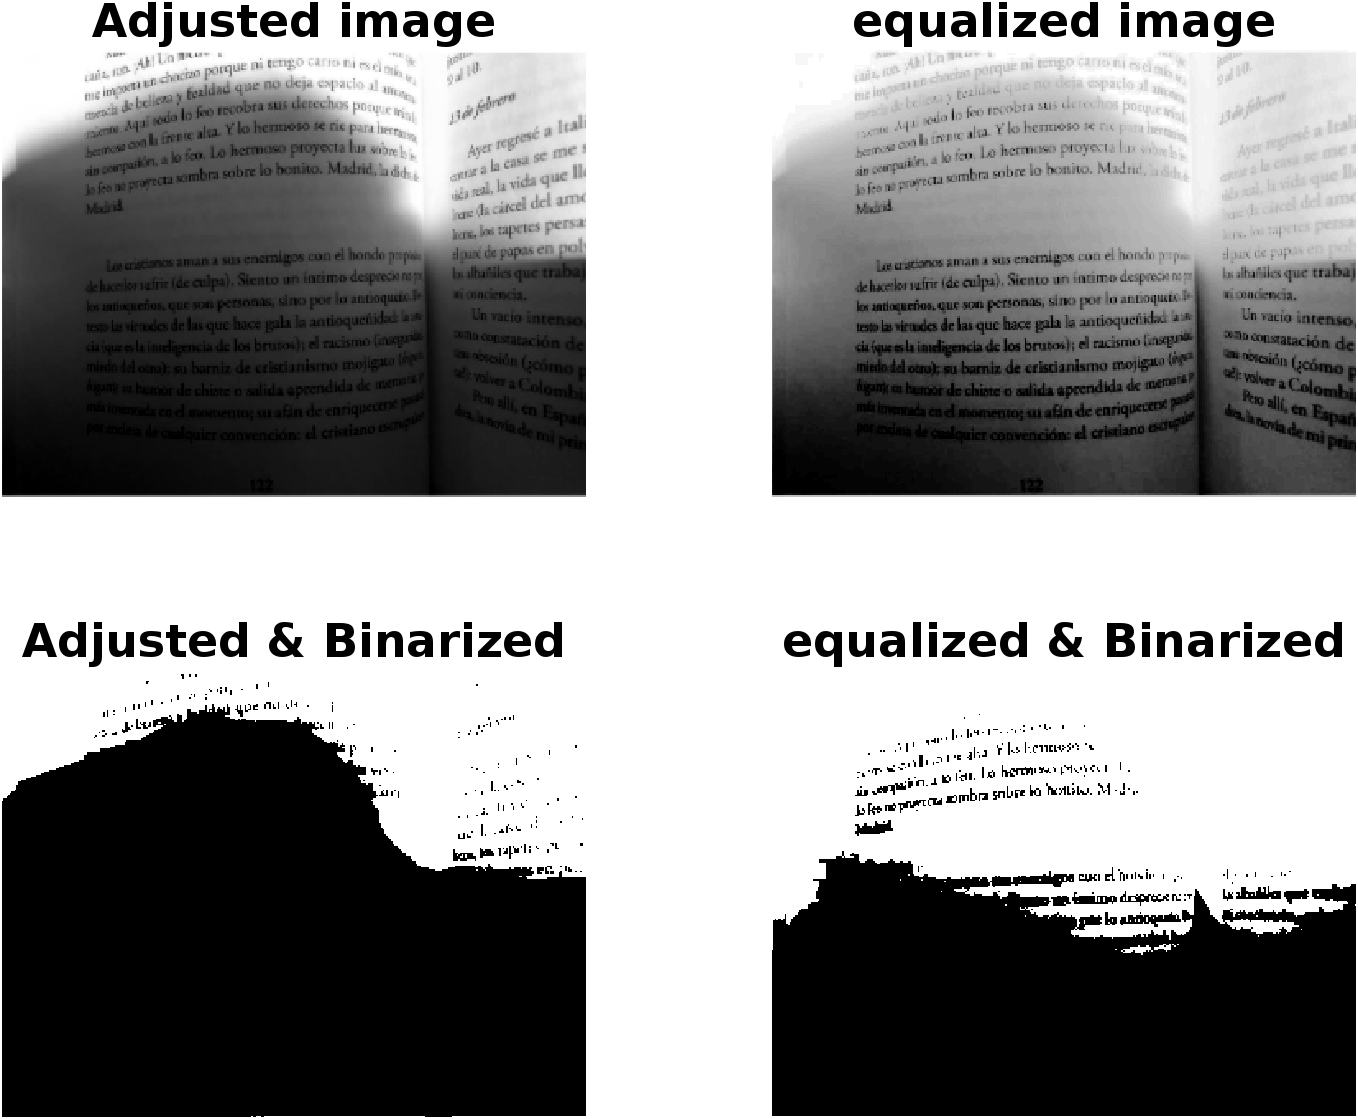
\includegraphics[width=0.50\linewidth]{Images/Figure 8.png} 
    \caption{Binarization results on grayscale images .}
    \label{fig:dynamic_range_expansion}
\end{figure}

\begin{figure}[H]
    \centering
    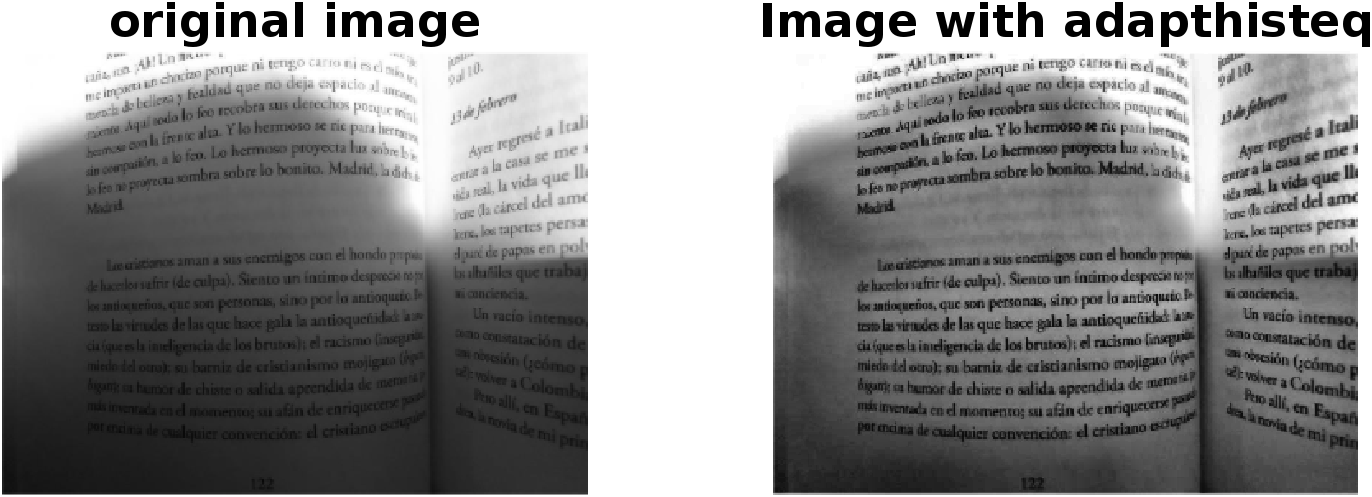
\includegraphics[width=0.50\linewidth]{Images/Figure 9.png} 
    \caption{Adaptive Histogram Equalization results on grayscale images.}
    \label{fig:dynamic_range_expansion}
\end{figure}


\subsection{Color Image Processing}
\textbf{Task 1:} Channel Extraction:\\
The red channel provided the clearest contrast for isolating the carrots in carottes.png. The green and blue channels were less effective due to their weaker contrast in the image.

\begin{figure}[H]
    \centering
    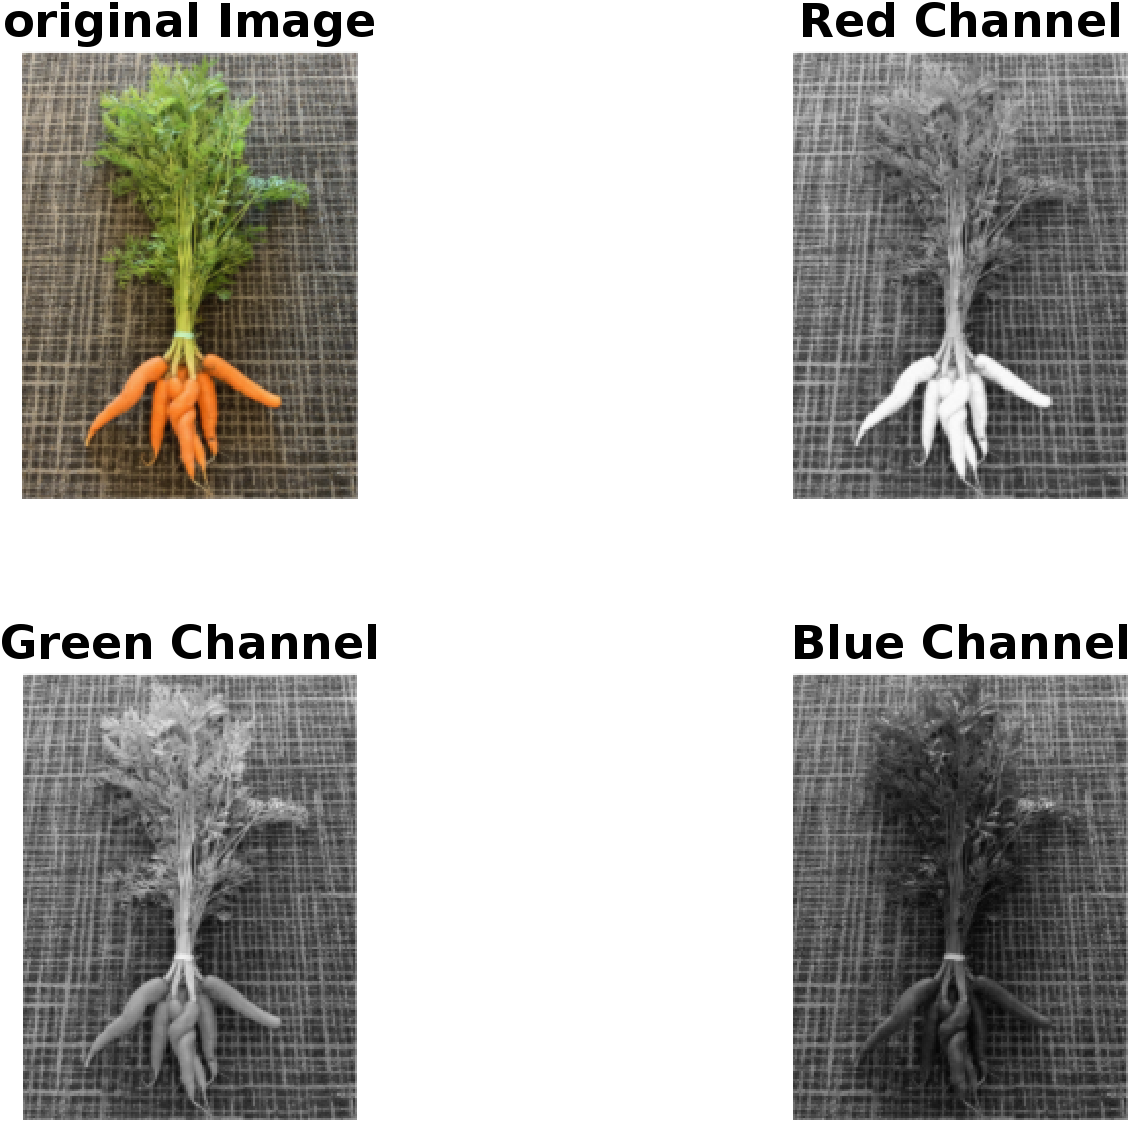
\includegraphics[width=0.50\linewidth]{Images/Figure 10.png} 
    \caption{Channel Extraction results.}
    \label{fig:dynamic_range_expansion}
\end{figure}

\begin{figure}[H]
    \centering
    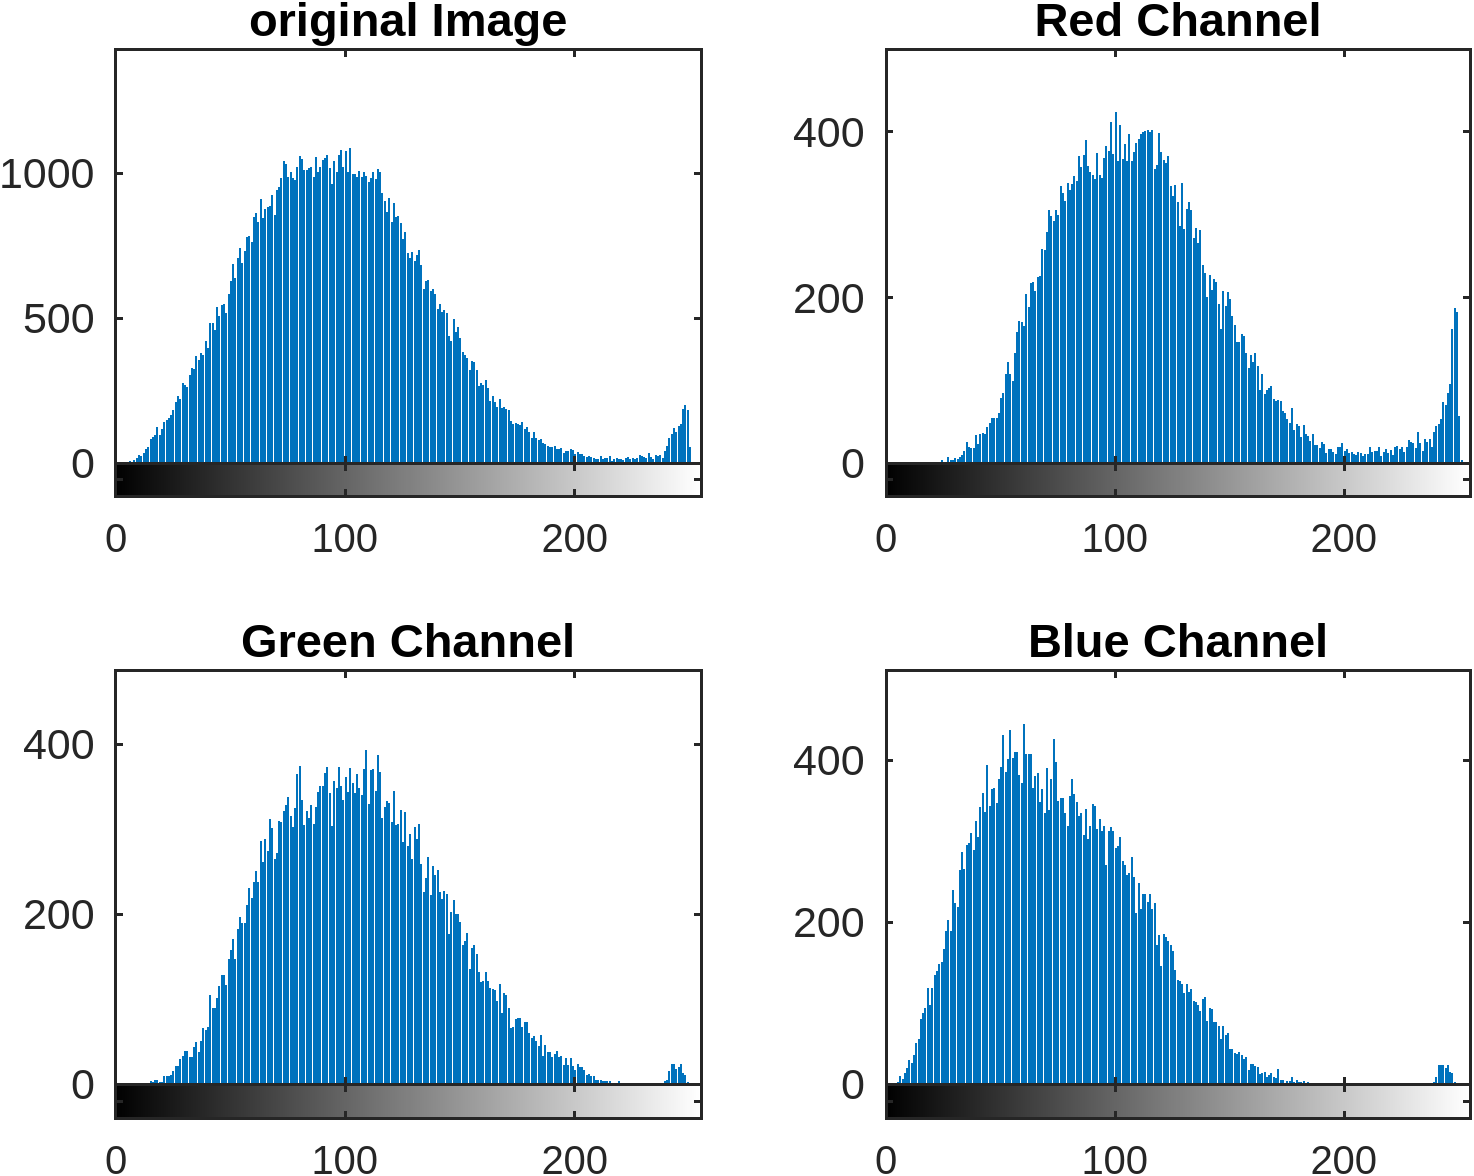
\includegraphics[width=0.50\linewidth]{Images/Figure 11.png} 
    \caption{Channel Extraction Histograms.}
    \label{fig:dynamic_range_expansion}
\end{figure}

\textbf{Task 2:} Segmentation\\
Automatic thresholding using graythresh effectively isolated the carrots, though manual thresholding, based on visual inspection of histograms, allowed for more precise control over segmentation, especially in areas of similar color.

\begin{figure}[H]
    \centering
    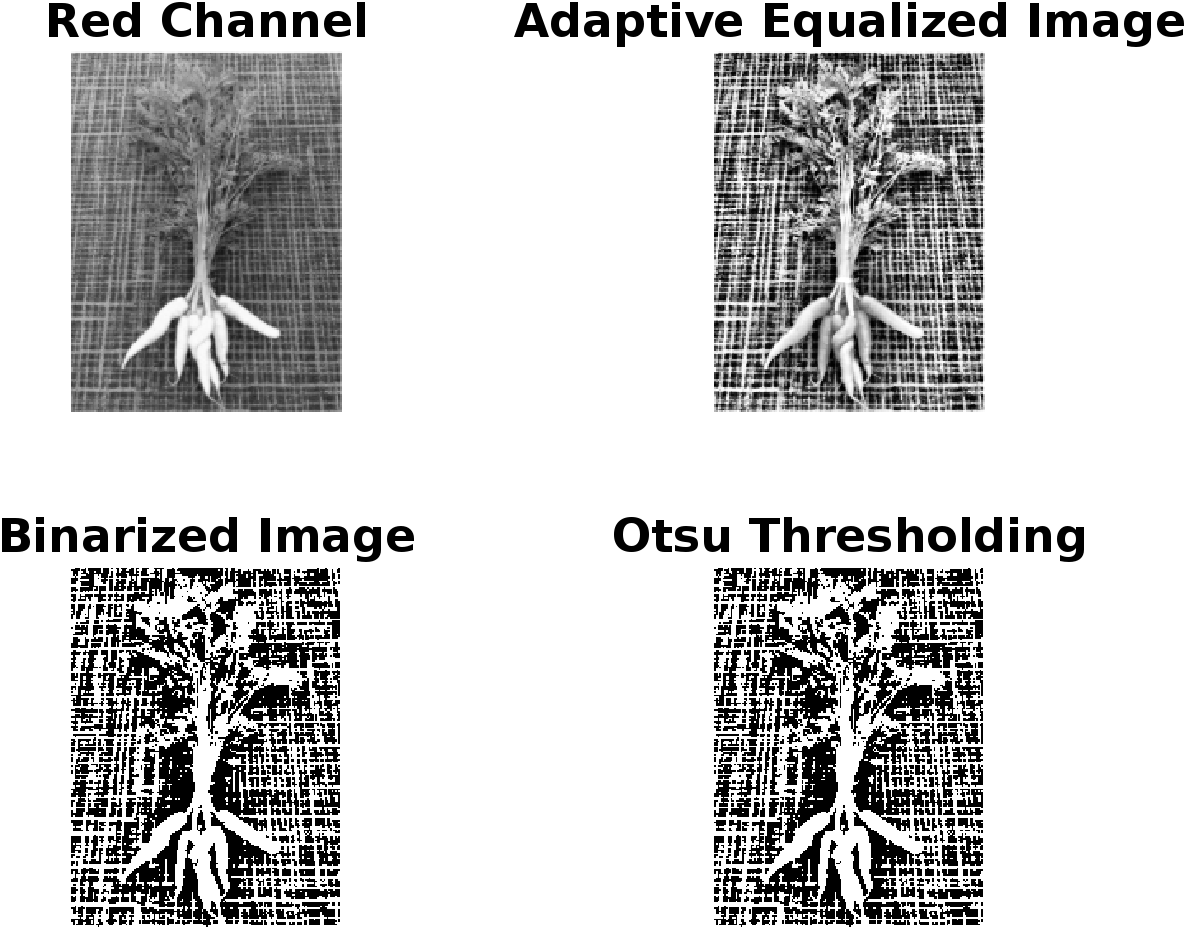
\includegraphics[width=0.50\linewidth]{Images/Figure 12.png} 
    \caption{Segmentation results on grayscale images.}
    \label{fig:dynamic_range_expansion}
\end{figure}

\section{Discussion}
The results highlight the strengths and limitations of the image enhancement techniques tested:

\textbf{Dynamic Range Expansion:} This method is simple and useful for enhancing general contrast but may not be sufficient for images with uneven lighting, where details in shadows or highlights might still be unclear.

\textbf{Histogram Equalization:} Effective for overall contrast enhancement, this method improves image clarity, especially in dimly lit regions. However, it may produce unnatural contrasts in some areas, especially when applied to complex images.

\textbf{Adaptive Histogram Equalization:} By adjusting the image locally, this method performs best in images with non-uniform lighting, making it ideal for applications such as text extraction and medical imaging. It was the most effective for enhancing book.png and segmenting the text.

\textbf{Color Channel Extraction and Segmentation:} Extracting the red channel was the most successful for isolating the carrots in carottes.png. While automatic thresholding worked well, manual thresholding gave better control over the final result.

%%%%%%%%%%%%%%%%%%%%%%%%%%%%%%%%%%%%%%%%%%%%%%%%%%%%%%%%%%%%%%%%%%%%%%%%%%
\section{Conclusion}
In conclusion, adaptive histogram equalization emerged as the most effective technique for enhancing images with uneven lighting, significantly improving detail and contrast. Additionally, color channel segmentation proved invaluable for isolating objects in complex, multi-colored images, demonstrating its importance in targeted image analysis.

\section{Appendix}
To maintain clarity and focus on the primary objectives, not all result images and code snippets are included in this report. However, the full set of results, including intermediate images, and the complete source code are available in the corresponding GitHub repository.
\href{https://github.com/aelmahraoui/MSc-IPS/tree/main/01.%201st%20semester/Computer%20Vision/Assignments/A01}{Github Repository Link}





%%%%%%%%%%%%%%%%%%%%%%%%%%%%%%%%%%%%%%%%%%%%%%%%%%%%%%%%%%%%%%%%%%%%%%%%%%

% \bibliographystyle{ieeetr}
% \bibliography{references.bib}

\end{multicols}
\end{document}
